\documentclass[tikz,border=2mm]{standalone}
\usetikzlibrary{shapes.geometric, arrows}

% Define block styles
\tikzstyle{startstop} = [rectangle, rounded corners, minimum width=3cm,
    minimum height=1cm,text centered, draw=black, fill=red!30]
\tikzstyle{process} = [rectangle, minimum width=3cm, minimum height=1cm,
    text centered, draw=black, fill=blue!30]
\tikzstyle{decision} = [diamond, minimum width=3cm, minimum height=1cm,
    text centered, draw=black, fill=green!30]
\tikzstyle{arrow} = [thick,->,>=stealth]

\begin{document}
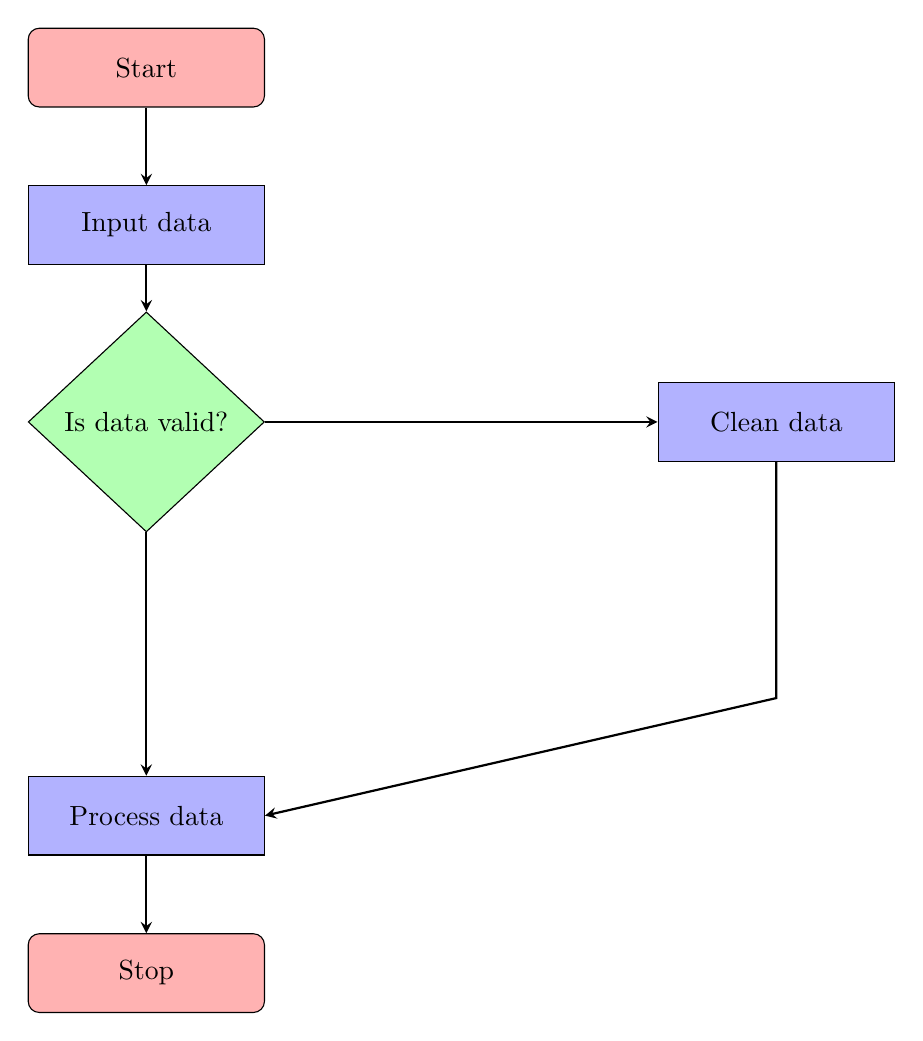
\begin{tikzpicture}[node distance=2cm]

% Nodes
\node (start) [startstop] {Start};
\node (in1) [process, below of=start] {Input data};
\node (dec1) [decision, below of=in1, yshift=-0.5cm] {Is data valid?};
\node (pro1) [process, right of=dec1, xshift=6cm] {Clean data};
\node (out1) [process, below of=dec1, yshift=-3cm] {Process data};
\node (stop) [startstop, below of=out1] {Stop};

% Arrows
\draw [arrow] (start) -- (in1);
\draw [arrow] (in1) -- (dec1);
\draw [arrow] (dec1.east) -- ++(2cm,0) -- (pro1.west);
\draw [arrow] (pro1.south) -- ++(0,-3cm) -- (out1.east);
\draw [arrow] (dec1.south) -- (out1.north);
\draw [arrow] (out1) -- (stop);

\end{tikzpicture}
\end{document}